
\chapter{Метод исследования}

\section{Введение}


Представленное в диссертационной работе исследование выполнено методом прямого численного моделирования. 


During the last decades, direct numerical simulations (DNS) have been recognized as a powerful and reliable tool for studying the basic physics of turbulence. 


\section{Математическая постановка задачи}

Рассматривается течение вязкой несжимаемой жидкости в прямой трубе круглого сечения. Жидкость считается однородной --- её плотность $\rho$ и вязкость $\mu$ во всем объеме трубы постоянны. Движение вызывается внешним градиентом давления, направленным вдоль трубы.


Поле скорости $\v(\x,t)$ удовлетворяет уравнению несжимаемости
\begin{equation} \label{eq0}
\nabla \cdot \v = 0.
\end{equation}

Движение жидкости описывается уравнениями Навье-Стокса, которые для несжимаемой жидкости имеют вид
\begin{equation} \label{NSeq_dynamic}
\pd{\v}{t} = - (\v, \nabla) \v - \frac{1}{\rho}\nabla P + \frac{\mu}{\rho} \nabla^2 \v.
\end{equation}
Здесь $P = P(\x,t)$ --- поле давления. Уравнения решаются в цилиндрической системе координат $(x,r,\theta)$, где $x$ --- продольное, $r$ --- радиальное и $\theta$ --- угловое направления, $t$ --- время. 


На твердой стенке трубы радиуса $R$ ставятся условия прилипания
\begin{equation} \label{bc0}
\v = 0 \text{, при } r = R.
\end{equation}
В направлении движения устанавливаются условие периодичности с периодом $L_x$. Давление $P$, непосредственно, периодическим не является. Оно представляется в виде суммы периодической $p$ и линейной вдоль трубы $Dx$ составляющих. Подстановка $P = p + Dx$ в \eqref{NSeq_dynamic} дает уравнение
\begin{equation} \label{NSeq_periodic}
\pd{\v}{t} = - (\v, \nabla) \v - \frac{D}{\rho}\i - \frac{1}{\rho}\nabla p + \frac{\mu}{\rho} \nabla^2 \v.
\end{equation}
Здесь $\i$ -- единичный орт, направленный вдоль трубы. В уравнении \eqref{NSeq_periodic} все переменные удовлетворяют условию периодичности вдоль трубы
\begin{equation} \label{bc1}
[\v, p](x,r,\theta,t) = [\v, p](x+L_x,r,\theta,t).
\end{equation}

Величина $D$ представляет собой внешний градиент давления, который определяется из условия постоянства расхода жидкости, протекающей через трубу. Постановка задачи может быть легко обобщена на случай наличия внешних потенциальных сил $\F = \nabla U$. За $D$ в этом случае следует обозначить разность внешнего градиента давления и средней вдоль трубы составляющей $F_x$. Не вошедшая в $D$ часть $\F$ потенциальна. Разность периодической вдоль трубы части давления и её потенциала составляет $p$. 

Поставленная задача, определяемая уравнениями \eqref{eq0}, \eqref{bc0}, \eqref{NSeq_periodic}, \eqref{bc1}, имеет единственное решение для каждого начального поля скорости $\v_0(\x)$, удовлетворяющего условию несжимаемости \eqref{eq0}. Известно аналитическое решение задачи, называемое течением Пуазейля, соответствующее ламинарному режиму течения. Оно существует при всех значениях параметров и задается формулой
\begin{equation}
\v = (U (1 - (r / R)^2), 0, 0).
\end{equation}
Здесь величина $U = - D R^2\mu^{-1}/4 $ определяется по градиенту давления $D$ и соответствует максимальной скорости в ламинарном течении, которую оно достигает на оси трубы. Несложно показать, что средняя скорость течения $U_q$, вычисленная как отношение расхода к площади сечения трубы, в этом случае равна $U/2$. 


В работе все вычисления выполняются в безразмерных переменных. В качестве масштабов выступают радиус трубы $R$, максимальная скорость в ламинарном течении $U$ и плотность жидкости $\rho$. Переход к безразмерным единицам измерения, обозначенным штрихами, выполняется по формулам
\begin{equation} \label{dim_less_eqs}
R x' = x,  R r' = r, RU^{-1} t' = t, U\v' = \v , \rho U^2 p' = p, \rho U^2 R^{-1} D' = D, R L'_x = L_x.
\end{equation}

В безразмерных единицах измерения уравнения \eqref{eq0}, \eqref{bc0}, \eqref{NSeq_periodic}, \eqref{bc1} принимают вид (штрихи опущены):
\begin{equation}\label{eq0_Re}
\nabla \cdot \v = 0,
\end{equation}
\begin{equation}\label{NSeq_Re}
\pd{\v}{t} =  - \i D - (\v, \nabla) \v - \nabla p + \frac{1}{\Re} \nabla^2 \v,
\end{equation}
\begin{equation}\label{bc0_Re}
\v = 0 \text{ при } r = 1,
\end{equation}
\begin{equation}\label{bc1_Re}
[\v, p](x,r,\theta,t) = [\v, p](x+L_x,r,\theta,t)
\end{equation}
Здесь $\Re = \rho R U / \mu$ --- число Рейнольдса, один из двух параметров системы. Вторым параметром является $L_x$. Величина $D$ подбирается из условия постоянства расхода так, что $U_q = 1/2$ в безразмерных единицах. В случае ламинарного течения она выражается в явном виде: $D = - 4 \Re^{-1}$. Ламинарное течение в безразмерном виде задается более простым выражением 
\begin{equation}
\v = (1 - r^2, 0, 0).
\end{equation}

Многие авторы вводят число Рейнольдса иначе, через расходную скорость $U_q$ и диаметр трубы $D$. Несложно показать, что значение числа Рейнольдса, введенного таким образом, совпадает со значением числа Рейнольдса, введенного выше. Однако, например, единица измерения времени $DU_q^{-1}$ в этом случае увеличивается в 4 раза.

В процессе решения задачи возникает необходимость перехода в подвижную систему координат. Выполняя переход, удобно сохранить в качестве тела, относительно которого определяются скорости, стенки трубы. В этом случае граничные условия и значения скорости не зависят от системы отсчета, но в уравнении движения \eqref{NSeq_Re} возникает новое слагаемое
\begin{equation}\label{NSeq_cf}
\pd{\v}{t} = c_f \pd{\v}{x} - (\v, \nabla) \v - \i D - \nabla p + \frac{1}{\Re} \nabla^2 \v. 
\end{equation}
Возникшее слагаемое отвечает за перенос решения вдоль трубы со скоростью $-c_f$, где $c_f = c_f(t)$ --- скорость перемещения системы координат, может быть функцией времени. Уравнение неразрывности \eqref{eq0_Re} при переходе, выполненном таким образом, не меняется. 


Поставленная задача сформулирована традиционным образом для прямого расчета турбулентных потоков в прямых каналах. В такой постановке удается воспроизводить характеристики течения, устанавливающегося на большом удалении от входа в трубу, решая уравнения лишь в ограниченной расчетной области. Условие периодичности освобождает от необходимости устанавливать условия на входе и выходе из трубы. В тоже время, увеличивая длину периода $L_x$, можно минимизировать влияние этого условия на поток. Для того, чтобы иметь возможность воспроизвести в расчете локализованные турбулентные структуры, необходимо выбирать длину $L_x$ достаточно большой, не менее $40$ диаметров трубы. 


\section{Численный метод}

\begin{comment}
Поставленная задача решается численно конечно-разностным методом \cite{nikitin2006method}. Метод формулируется относительно уравнения движения \eqref{NSeq_Re}, преобразованного к виду 
\begin{equation}\label{NSeq_om}
\pd{\v}{t} = - \i D + \v \times \om - \nabla P - \frac{1}{\Re} \rot \om
\end{equation}
Здесь $\om = \rot \v$ --- вектор завихренности, посчитанный по полю скорости $\v$, $P = p + |\v|^2/2$ --- полное кинематическое давление. Эквивалентность уравнений \eqref{NSeq_Re} и \eqref{NSeq_om} следует из векторных тождеств
\begin{equation*}
-(\v, \nabla) \v = \v \times \rot \v - \nabla |\v|^2/2,
\end{equation*}
\begin{equation*}
\nabla^2 \v = \grad \div \v - \rot \rot \v.
\end{equation*}
\end{comment}

Поставленная задача решается численно конечно-разностным методом \cite{Nikitin2006}, в цилиндрической системе координат $(x,r,\theta)$. Расчетная область в переменных $(x,r,\theta)$ имеет форму параллелепипеда
\begin{equation}
0 < x < L_x, 0 < r < 1, 0 < \theta < 2\pi.
\end{equation}
При решении уравнений в этих переменных необходимо дополнительно установить условия периодичности в направлении $\theta$ и ограниченности решения при $r=0$.

В переменных $(x,r,\theta)$ в расчетной области вводится прямоугольная система координат, однородная в направлениях $x$ и $\theta$. В радиальном направлении вводится растяжение сетки, что позволяет сгустить её вблизи стенки. Во всех расчетах, приведенных ниже, параметр растяжения выбран так, что размер ячейки в радиальном направлении около стенки в 4 раза меньше, чем в центре трубы. 

При дискретизации уравнений применен подход, при котором различные неизвестные определяются в различных точках сетки. Так, давление $p$ относится к центру ячеек. Компоненты вектора скорости $v_k$ относятся к центрам граней, нормальных к направлению $k$. В процессе счета и при анализе решений возникает необходимость вычисления завихренности $\omega$. Компоненты вектора завихренности $\omega_k$ относятся к центрам ребер, параллельных направлению $k$. При таком подходе говорят, что неизвестные определены на смещенных или разнесенных сетках. Он позволяет естественным образом ввести аппроксимацию уравнения второго порядка точности по пространству. 

Пространственная дискретизация введена таким образом, что сохраняется ряд важных консервативных свойств исходной системы. В частности, тождественно равна нулю дивергенция вязких слагаемых в \eqref{NSeq_Re}, что гарантирует, что это слагаемое не производит массы. Также тождественно равна нулю завихренность градиента давления, что обеспечивает отсутствие влияния давления на эволюцию завихренности непосредственно. 

При моделировании турбулентных течений важно аккуратно воспроизводить изменение кинетической энергии системы. Уравнение, описывающее его, возникает в результате скалярного умножения на $\v$ уравнений движения \eqref{NSeq_Re} с последующим суммированием по всей расчетной области. Важным свойством системы является то, что в уравнении Навье-Стокса для несжимаемой жидкости градиент давления и нелинейные слагаемые не производят кинетической энергии, а лишь перераспределяют уже существующую. В конечно-разностной постановке строго выполняются тождества, выражающие этот факт, выполненные при \eqref{eq0_Re}, \eqref{bc0_Re}, \eqref{bc1_Re}
$$
\int_V \v \cdot \nabla p\ d\tau= \int_V \nabla (\v p) d\tau = \int_{\Sigma} p v_n d\sigma = 0, 
$$
$$
\int_V \v \cdot (\v, \nabla) \v\ d\tau = \int_V (\v, \nabla)\frac{|\v|^2}{2}\ d\tau = \int_V \nabla (\v \frac{|\v|^2}{2}) d\tau = \int_{\Sigma} \frac{|\v|^2}{2} v_n d\sigma = 0.
$$
Здесь $V$ --- расчетная область, $\Sigma$ --- её граница, $v_n$ --- нормальная составляющая скорости на границе. Также строго выполняется дискретный аналог уравнения изменения полной кинетической энергии $E$, записанного в следующем виде
\begin{equation} \label{Eeq}
\d{E}{t} = - \frac{1}{2}DV - \frac{1}{\Re} \int_{V} |\omega|^2 d\tau,
\end{equation}
$$
E = \frac{1}{2}\int_{V} |\v|^2 d\tau.
$$
Изменение полной энергии происходит за счет внешнего градиента давления $D$ и вязкой диссипации. 

Интегрирование по времени выполняется полу-неявным методом Рунге-Кутты третьего порядка точности \cite{Nikitin2006third}. В силу нелинейности оператора Навье-Стокса реализовать полностью неявный метод продвижения по времени затруднительно. Однако наибольшая жесткость системы на достаточно подробных сетках вызвана вязкими слагаемыми. В силу их линейности они могут быть разрешены неявно в то время, как другие слагаемые в операторе Навье-Стокса разрешаются явно. Такой подход называется полу-неявным и позволяет существенно увеличить допустимый временной шаг в сравнении с явными методами. Реализованный алгоритм допускает автоматический выбор шага интегрирования исходя из условия сохранения локальной точности получаемого решения. Таким образом шаг интегрирования автоматически адаптируется к изменением в структуре течения, и не требует явного его задания во время счета. 

Неточность выполнения закона сохранения энергии в конечно-разностной постановку может быть следствием не только несовершенства пространственной дискретизации, но и в результате неточности выполнения интегрирования по времени. Метод Рунге-Кутты третьего порядка обладает важным свойством диссипативности --- неточности выполнения шага по времени могут вести лишь к потере кинетической энергии, но не её производству. 


На каждом шаге по времени возникает необходимость по известному полю скорости $\v$ определить давление $p$. Для этого необходимо решить уравнение Пуассона, возникающее в результате применения оператора дивергенции к уравнению движения \eqref{NSeq_Re} при условии несжимаемости \eqref{eq0_Re}, имеющее вид
\begin{equation}\label{Peq}
\nabla^2 p = \div \tilde \v,
\end{equation}
$$
\tilde \v = - (\v,\nabla)\v + \frac{1}{\Re}\nabla^2 \v. 
$$
Правая часть уравнения \eqref{Peq} известна. Давление также удовлетворяет условию периодичности в направлениях $x$ и $\theta$. На оси трубы значение давления ограничено. Условие на твердой стенке возникает в результате проектирования уравнения \eqref{NSeq_Re} на направление нормали $n$
$$
\pd{p}{n} = \tilde v_n.
$$


Простая геометрия расчетной области позволяет применять прямые методы решения возникающей линейной системы. Метод решения задачи для давления основан на применении быстрого преобразования Фурье в направлениях $x$ и $\theta$, в которых решение меняется периодическим образом и сетка имеет постоянный шаг. В радиальном направлении система решается методом прогонки. Общая сложность решения задачи для давления составляет $O(N \log N)$, где $N$ --- количество точек в сетке. Решение задачи для давления составляет основную вычислительную сложность используемого метода. 


\section{Реализация численного метода}

Программа, реализующая описанный выше численный метод, написана на языке fortran77. 

Программа была реализован на языке программирования фортран 77 Никитиным Н.В. (научным руководителем). Значительная часть кода, необходимого при анализе полученных результатов и управлении численными экспериментами, была реализована на скриптовом языке python. 


Помимо последовательного варианта программы был реалзован также параллельный. Для этого был использован интерфейс передачи сообщений (MPI), позволяющий обмениваться данными между различными копиями программы, запущенными в разном адресном пространстве. Реализация параллельной программы такова, что труба делится в проольном напрвени

В параллельной версии программы труба в проольном направлении делится на равные части, которые распределяются между процессами. Расчеты выполнялись на суперкомпьютерах <<Чебышев>> и <<Ломоносов>> суперкомпьютерного комплекса МГУ им. М.В.\,Ломоносова. 


\section{Методические расчеты}



Приводимые ниже результаты расчетов в диапазоне $1670\leqslant Re\leqslant 2800$ получены при $L_x=200$ с пространственным разрешением $2048 \times 64 \times 128$ в продольном, радиальном и угловом направлении соответственно. Расчеты на более грубой сетке $1024\times32\times64$ во всех рассмотренных случаях дают результаты совпадающие качественно и близкие количественно.

\begin{figure}[h]
\center{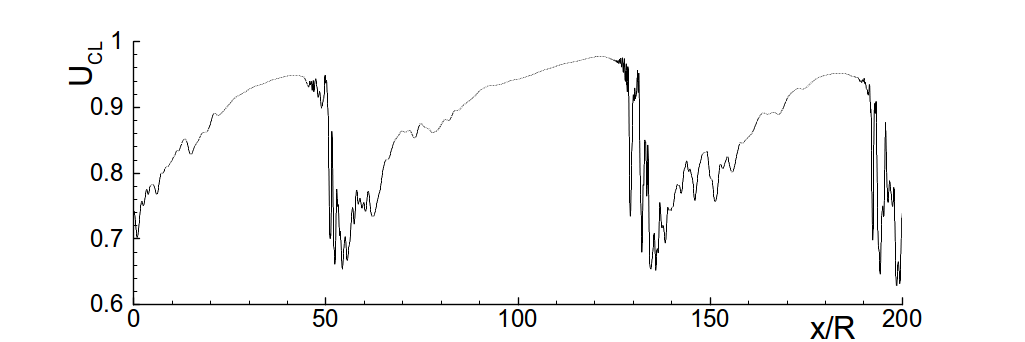
\includegraphics[width=0.9\linewidth]{exper2.png}}
\center{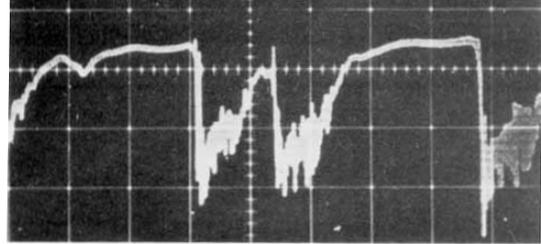
\includegraphics[width=0.68\linewidth]{exper3.png}}
\caption{Сравнение результатов численного расчета и эксперемента. Изображена скорость на оси трубы. Верхний график построен по результатам численного моделирования, выполнено Н.В. Никитиным методом, применяемым в работе. Нижный график получен в эксперименте Вигнанским и Чампайном, 1973 год.}
\label{exper_img}
\end{figure}

Стартуя с начальных данных в виде некоторого трехмерного возмущения течения Пуазейля, уравнения Навье--Стокса интегрируются до выхода решения на тот или иной режим. Установление решения, отвечающего турбулентному течению происходит в том случае, когда амплитуда начального возмущения достаточно велика, в противном случае возмущения затухают со временем, и решение в конечном итоге возвращается к ламинарному течению Пуазейля. Турбулентный режим за пределами диапазона переходных чисел Рейнольдса $Re\geqslant3000$ имеет вид статистически стационарного процесса и не зависит от конкретного вида начальных условий, при которых он был получен. Течение при этом однородно в продольном направлении, его статистические характеристики согласуются с имеющимися экспериментальными данными (см. рис. \ref{exper_img}). При $\Re\leqslant2600$ в распределении скорости вдоль трубы появляется неоднородность, которая при $\Re\lesssim2200$ приобретает форму двигающейся вдоль трубы цепочки из нескольких пространственно-локализованных структур, разделенных участками ламинарного течения. Конкретное число получающихся в решении турбулентных структур зависит от начальных условий. Кроме того, как было отмечено выше, это число может меняться в процессе эволюции в результате исчезновения или деления отдельных структур. Получаемые в расчетах пространственно-локализованные турбулентные структуры хорошо согласуются с наблюдаемыми в экспериментах турбулентными порывами, что позволяет нам пользоваться этим их наименованием. Отметим, что турбулентные порывы формируются и на некотором отрезке времени существуют в расчетах и при $Re<2000$, вплоть до $Re=1670$. Однако, в этом случае не только число порывов в пределах расчетной области, но и время их существования является случайной величиной и зависит от конкретных начальных условий. Представленная на фиг.~\ref{puffs_img} визуализация рассчитанных течений в диапазоне $1680\leqslant Re\leqslant2800$ демонстрирует эволюцию локализованных структур при изменении числа Рейнольдса.

\begin{figure}[h]
\center{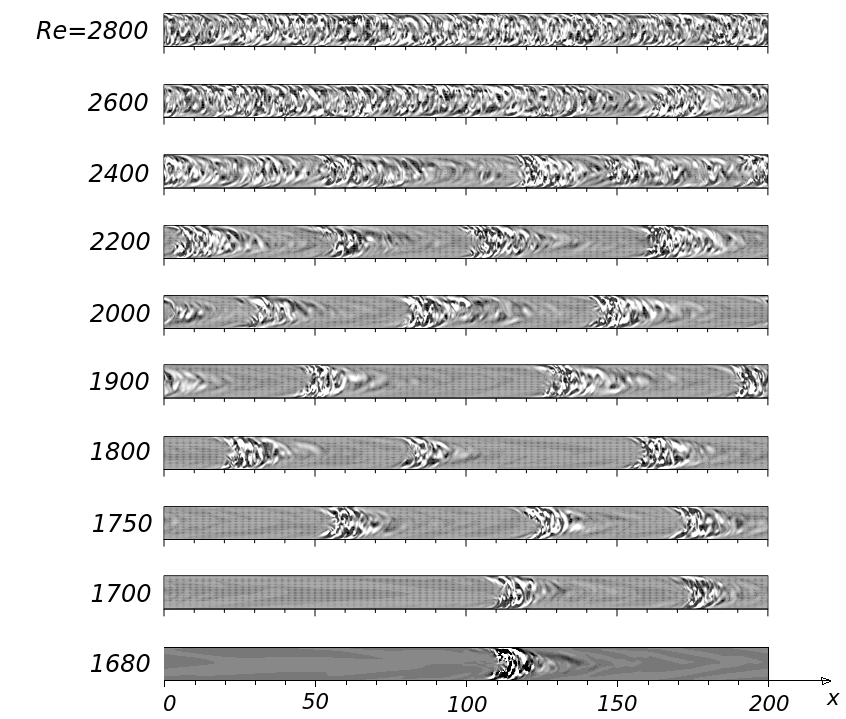
\includegraphics[width=1\linewidth]{puffs.png}}
\caption{Перемежаемый характер турбулентности в трубе в диапазоне переходных чисел Рейнольдса.}
\label{puffs_img}
\end{figure}

